\documentclass[a1paper, landscape, blockverticalspace=1cm, 14pt]{tikzposter}
\usepackage[utf8]{inputenc}
\usepackage{amsmath}
\usepackage{amsfonts}
\usepackage{amsthm}
\usepackage{amssymb}
\usepackage{mathrsfs}
\usepackage{graphicx}
\graphicspath{ {./images/} }
\usepackage{adjustbox}
\usepackage{enumitem}
\usepackage[backend=biber,style=numeric]{biblatex}
\usepackage{rutheme}
\usepackage{lipsum}
\usepackage{cancel}
\usepackage{mwe} % for placeholder images
\usepackage{graphbox}

\addbibresource{refs.bib}

% set theme parameters
\tikzposterlatexaffectionproofoff
\usetheme{RUTheme}
\usecolorstyle{RUStyle}

\usepackage[scaled]{helvet}
\renewcommand\familydefault{\sfdefault} 
\usepackage[T1]{fontenc}
\usepackage{hyperref}

\makeatletter
\def\title#1{\gdef\@title{\scalebox{\TP@titletextscale}{%
\begin{minipage}[t]{\linewidth}
\centering
#1
\par
\vspace{0.5em}
\end{minipage}%
}}}
\makeatother

\title{\Huge Construction/Operation of Two Hexacopters for Autonomous Landing}
\author{Joshua Springer}
\institute{Reykjavík University}
\titlegraphic{
\includegraphics[width=0.055\textwidth]{ru_logo_transparent.png}}

% begin document
\begin{document}
\maketitle
\centering
\begin{columns}

    \column{0.33}
    \block{Introduction}
    {
        \normalsize
        Two Tarot 680 hexacopters allow real world testing of autonomous navigation techniques.
        This project tests an autonomous landing algorithm based on computer vision and fiducial markers.\cite{AL_thesis}
        A landing pad is marked with fiducial markers which are recognized by the drone's onboard camera.
        The gimbal automatically aims the camera at the landing pad to track it during descent.
        The landing software then directs the drone to descend towards the landing pad.
    }

    \block{Components}
    {
        \normalsize
        All drone electronics (e.g. motors, speed controllers, propellers, power electronics, RC Receiver, telemetry radio) are mounted on the Tarot 680 Pro hexacopter body.
        A Raspberry Pi 3 B+ runs ArduPilot and generates software-level control commands.
        It has a Navio2 hat which provides IMU data, sends low-level control signals to the speed controllers and the camera's gimbal, and receives manual control signals from the RC system.
        A companion board handles image analysis and estimates the pose of the drone relative to the landing pad.
        A radio telemetry system provides real time data to a ground control station.

        \vspace{0.5cm}
        \begin{tikzfigure}%[Hardware Overview]
            \includegraphics[width=0.45\linewidth]{jetson_electronics}
            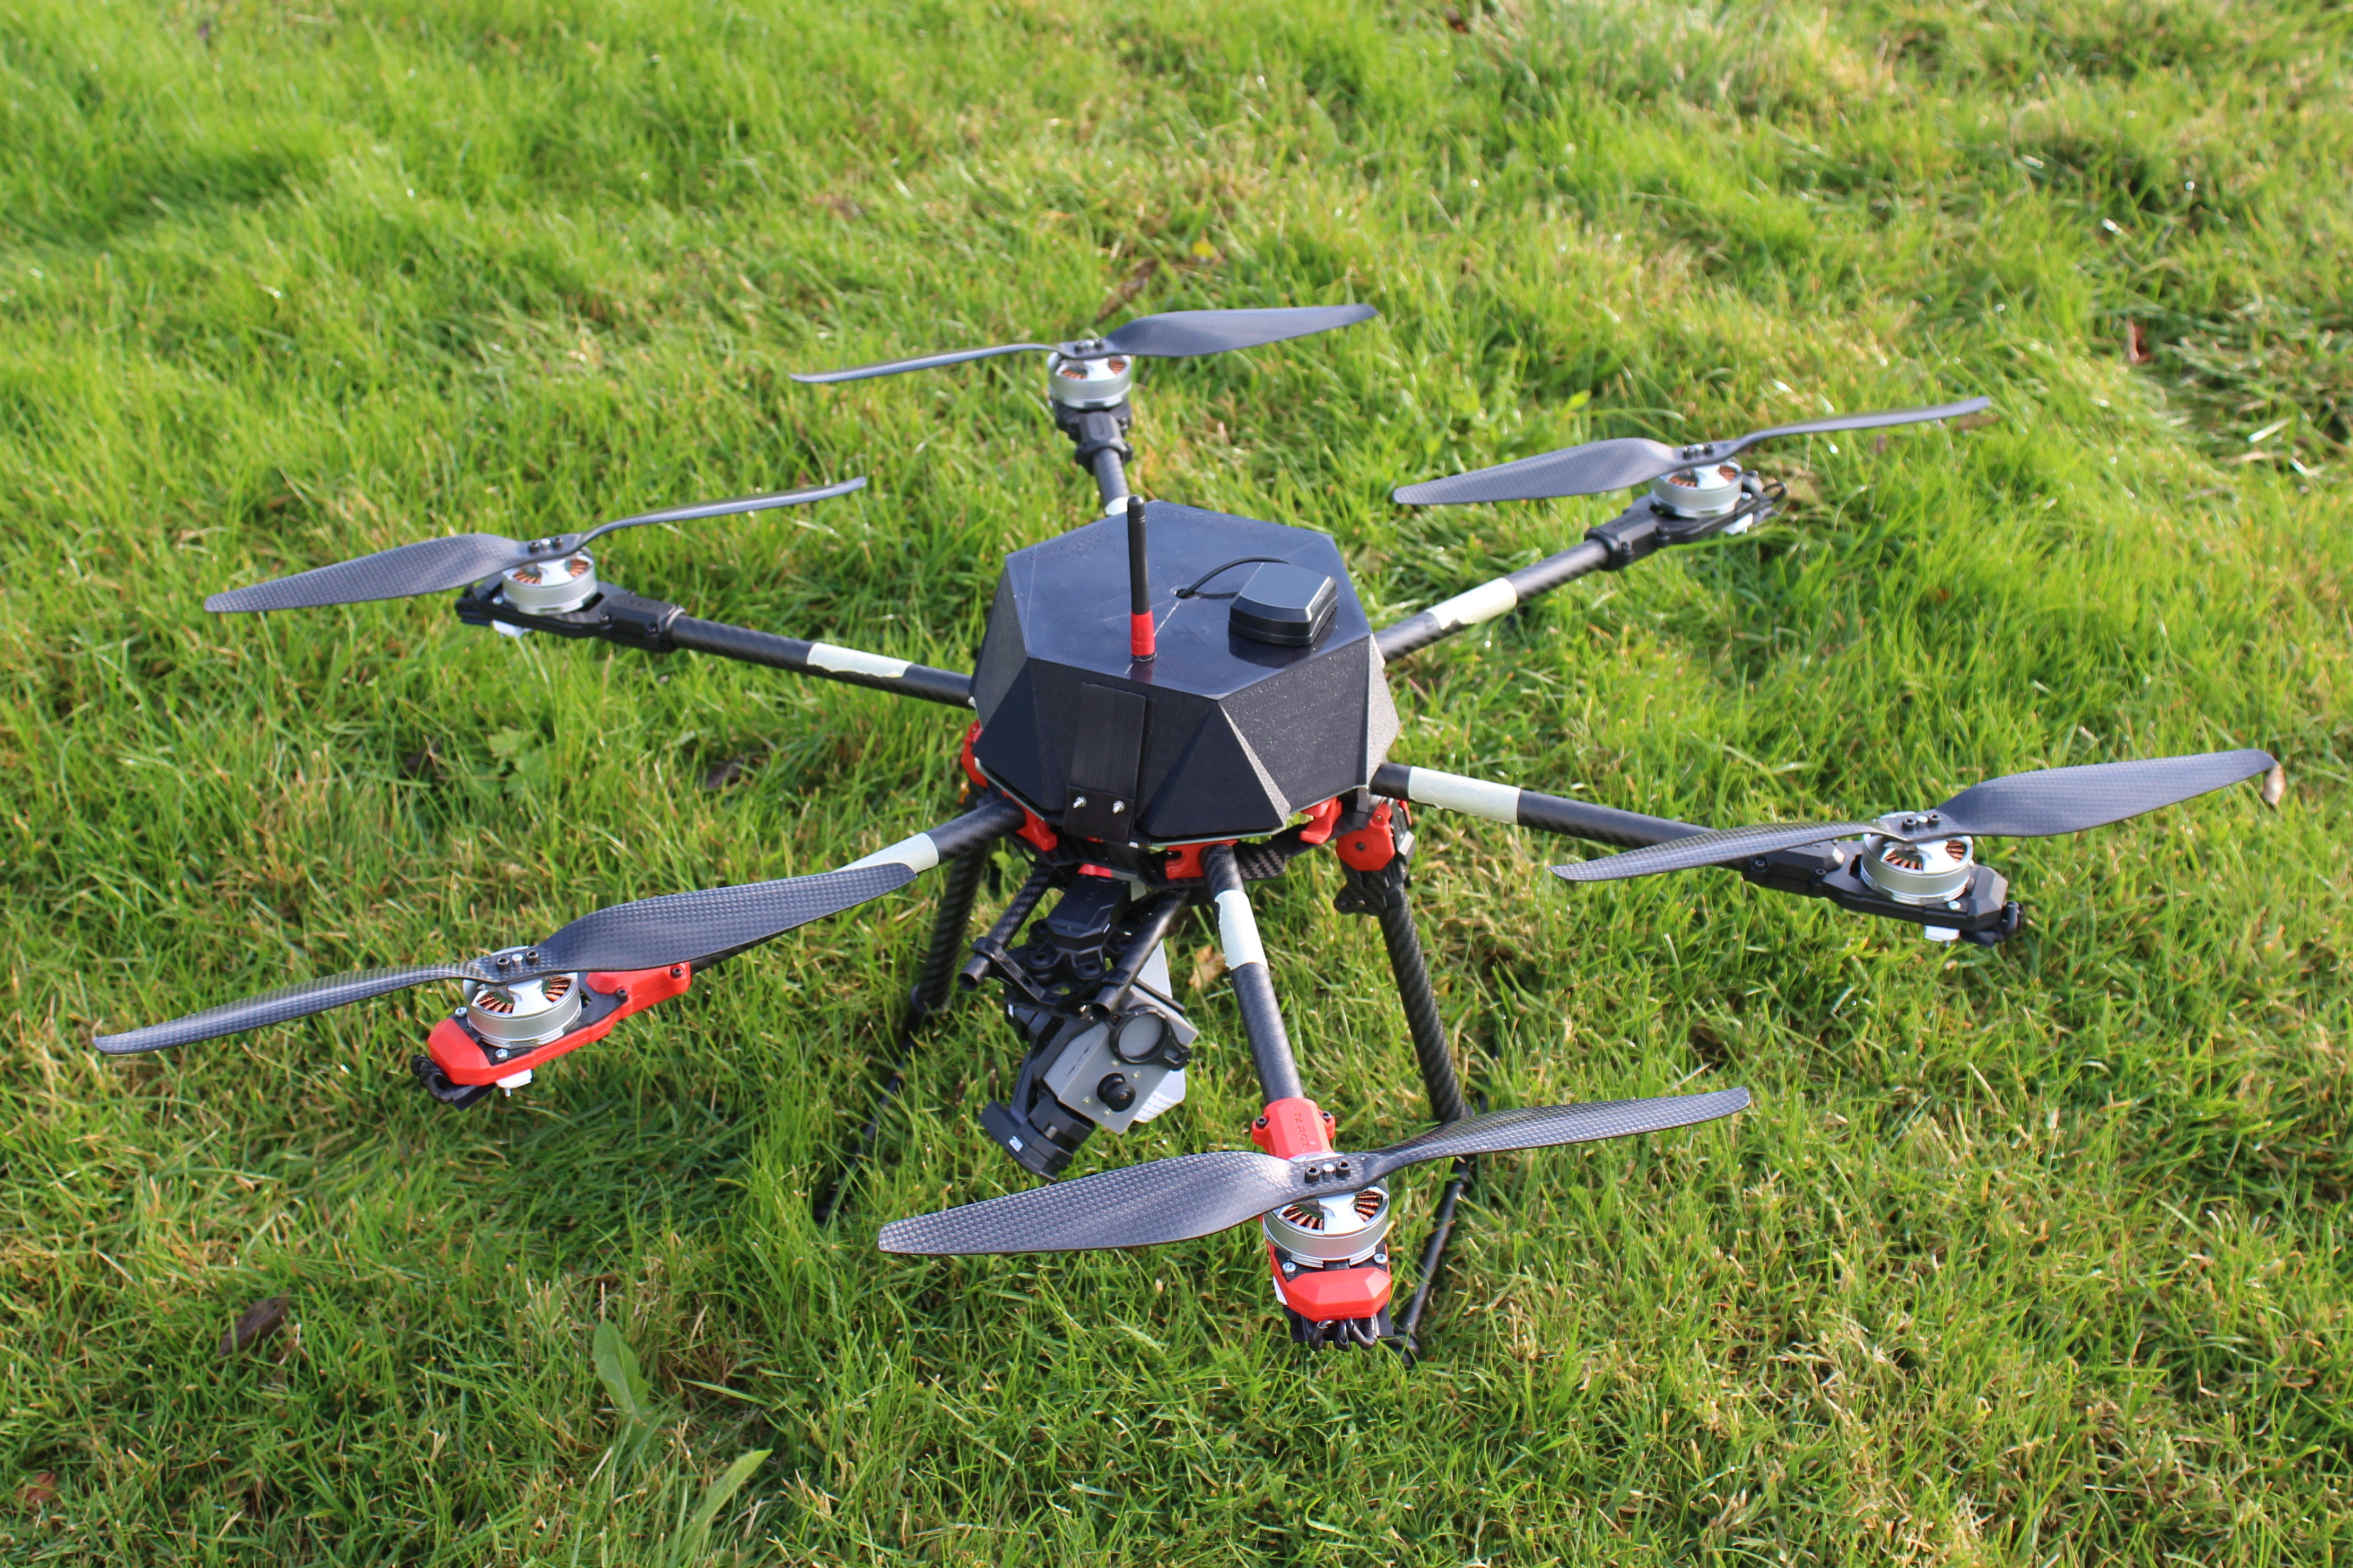
\includegraphics[width=0.45\linewidth]{jetson_drone.jpg}
        \end{tikzfigure}

        The Raspberry Pi runs a version of Raspbian Linux that is adapted for the Navio 2 hat. Together these create a flight controller, which communicates with the companion board via ROS using Ethernet over USB.
        The companion board analyzes video from the camera to detect the landing pad, aims the camera at the detected marker(s), estimates the pose of the drone relative to the landing pad, and then sends a target position to the flight controller.
        In autonomous flight mode, the flight controller flies the drone towards the target position in order to safely approach the landing pad.
        The two drones differ in their companion boards: one has an NVIDIA Jetson Nano, and the other has a Google Coral Dev.
    }

    \block{3D-Printed Components}
    {
        \normalsize
        A canopy from Thingiverse was 3D printed to cover the electronics.
        Component mounting plates were designed in OpenSCAD and provide a flat, secure surface to mount the electronics to the drone, as well as a hinge for the canopy.
        The camera cases also provide a way to mount the camera modules in the gimbal.

        \begin{tikzfigure}[Top right to bottom left - canopy, component mounting plate, Coral camera case, Jetson Nano camera case.]
            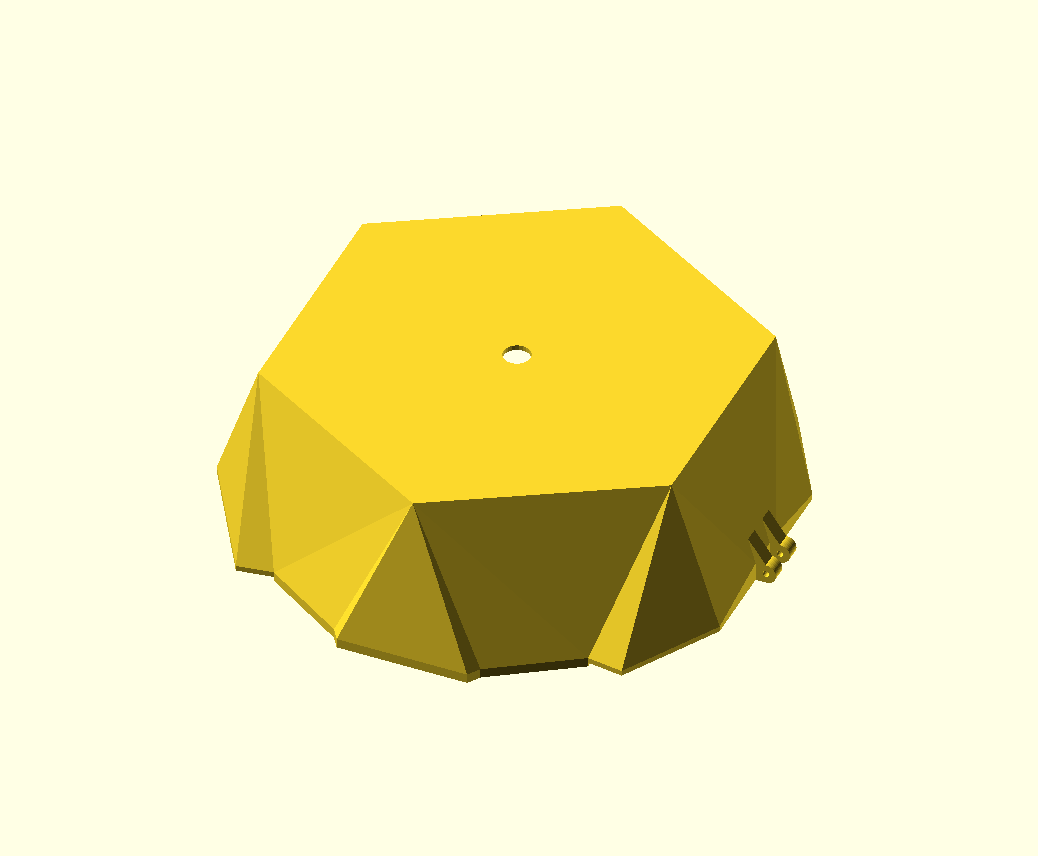
\includegraphics[width=0.4\linewidth]{canopy.png}
            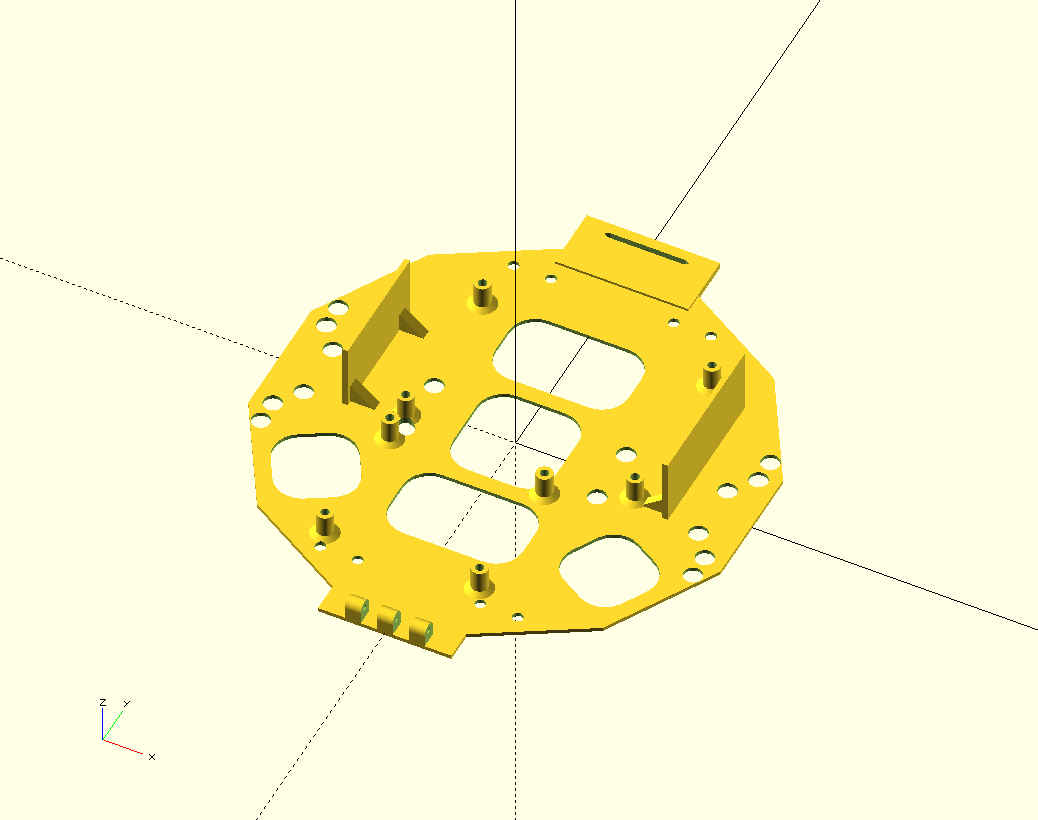
\includegraphics[width=0.4\linewidth]{component_mounting_plate}
            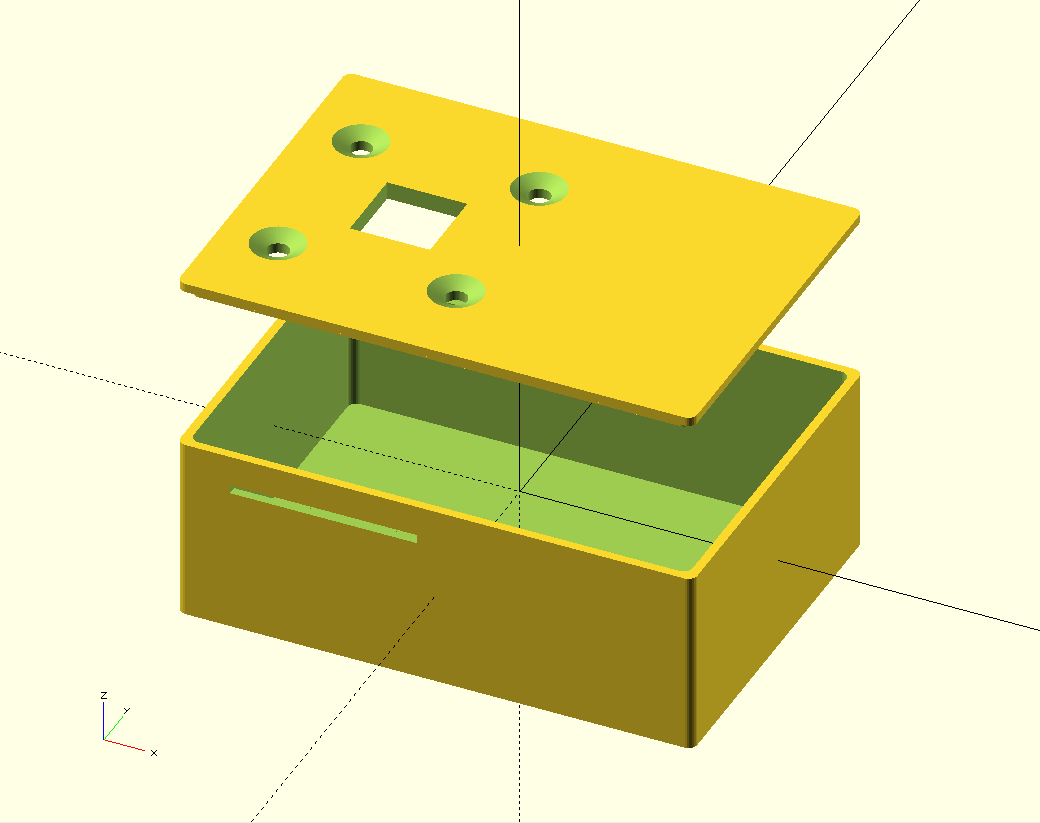
\includegraphics[width=0.4\linewidth]{coral_case.png}
            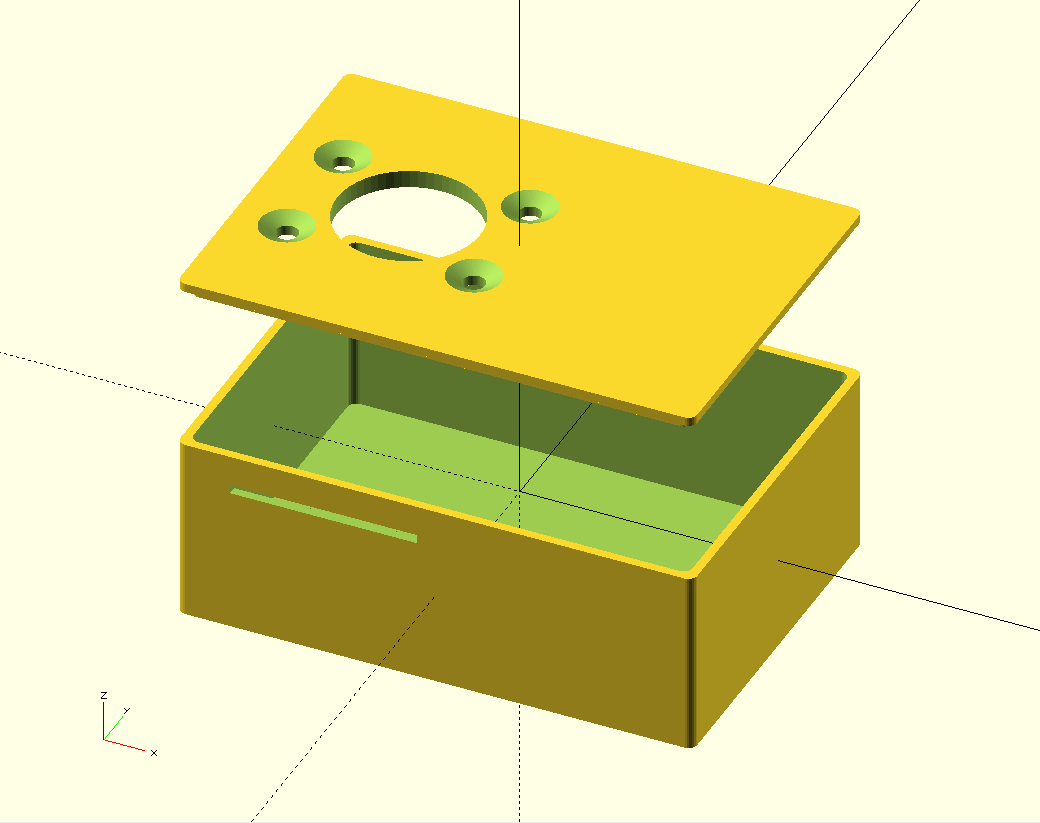
\includegraphics[width=0.4\linewidth]{nano_case.png}
        \end{tikzfigure}
    }

    \column{0.33}
    \block{Power and Data Flow}
    {
        \normalsize
        The drones have two isolated power systems - an 11.1V system (regulated to 5V by the BEC) for the electronics, and a 22.2V system for the motors and gimbal.
        This is because the electronics require a very stable power source to function reliably, and the motors can suddenly draw large currents, reducing the apparent voltage unpredictably.
        \begin{tikzfigure}
            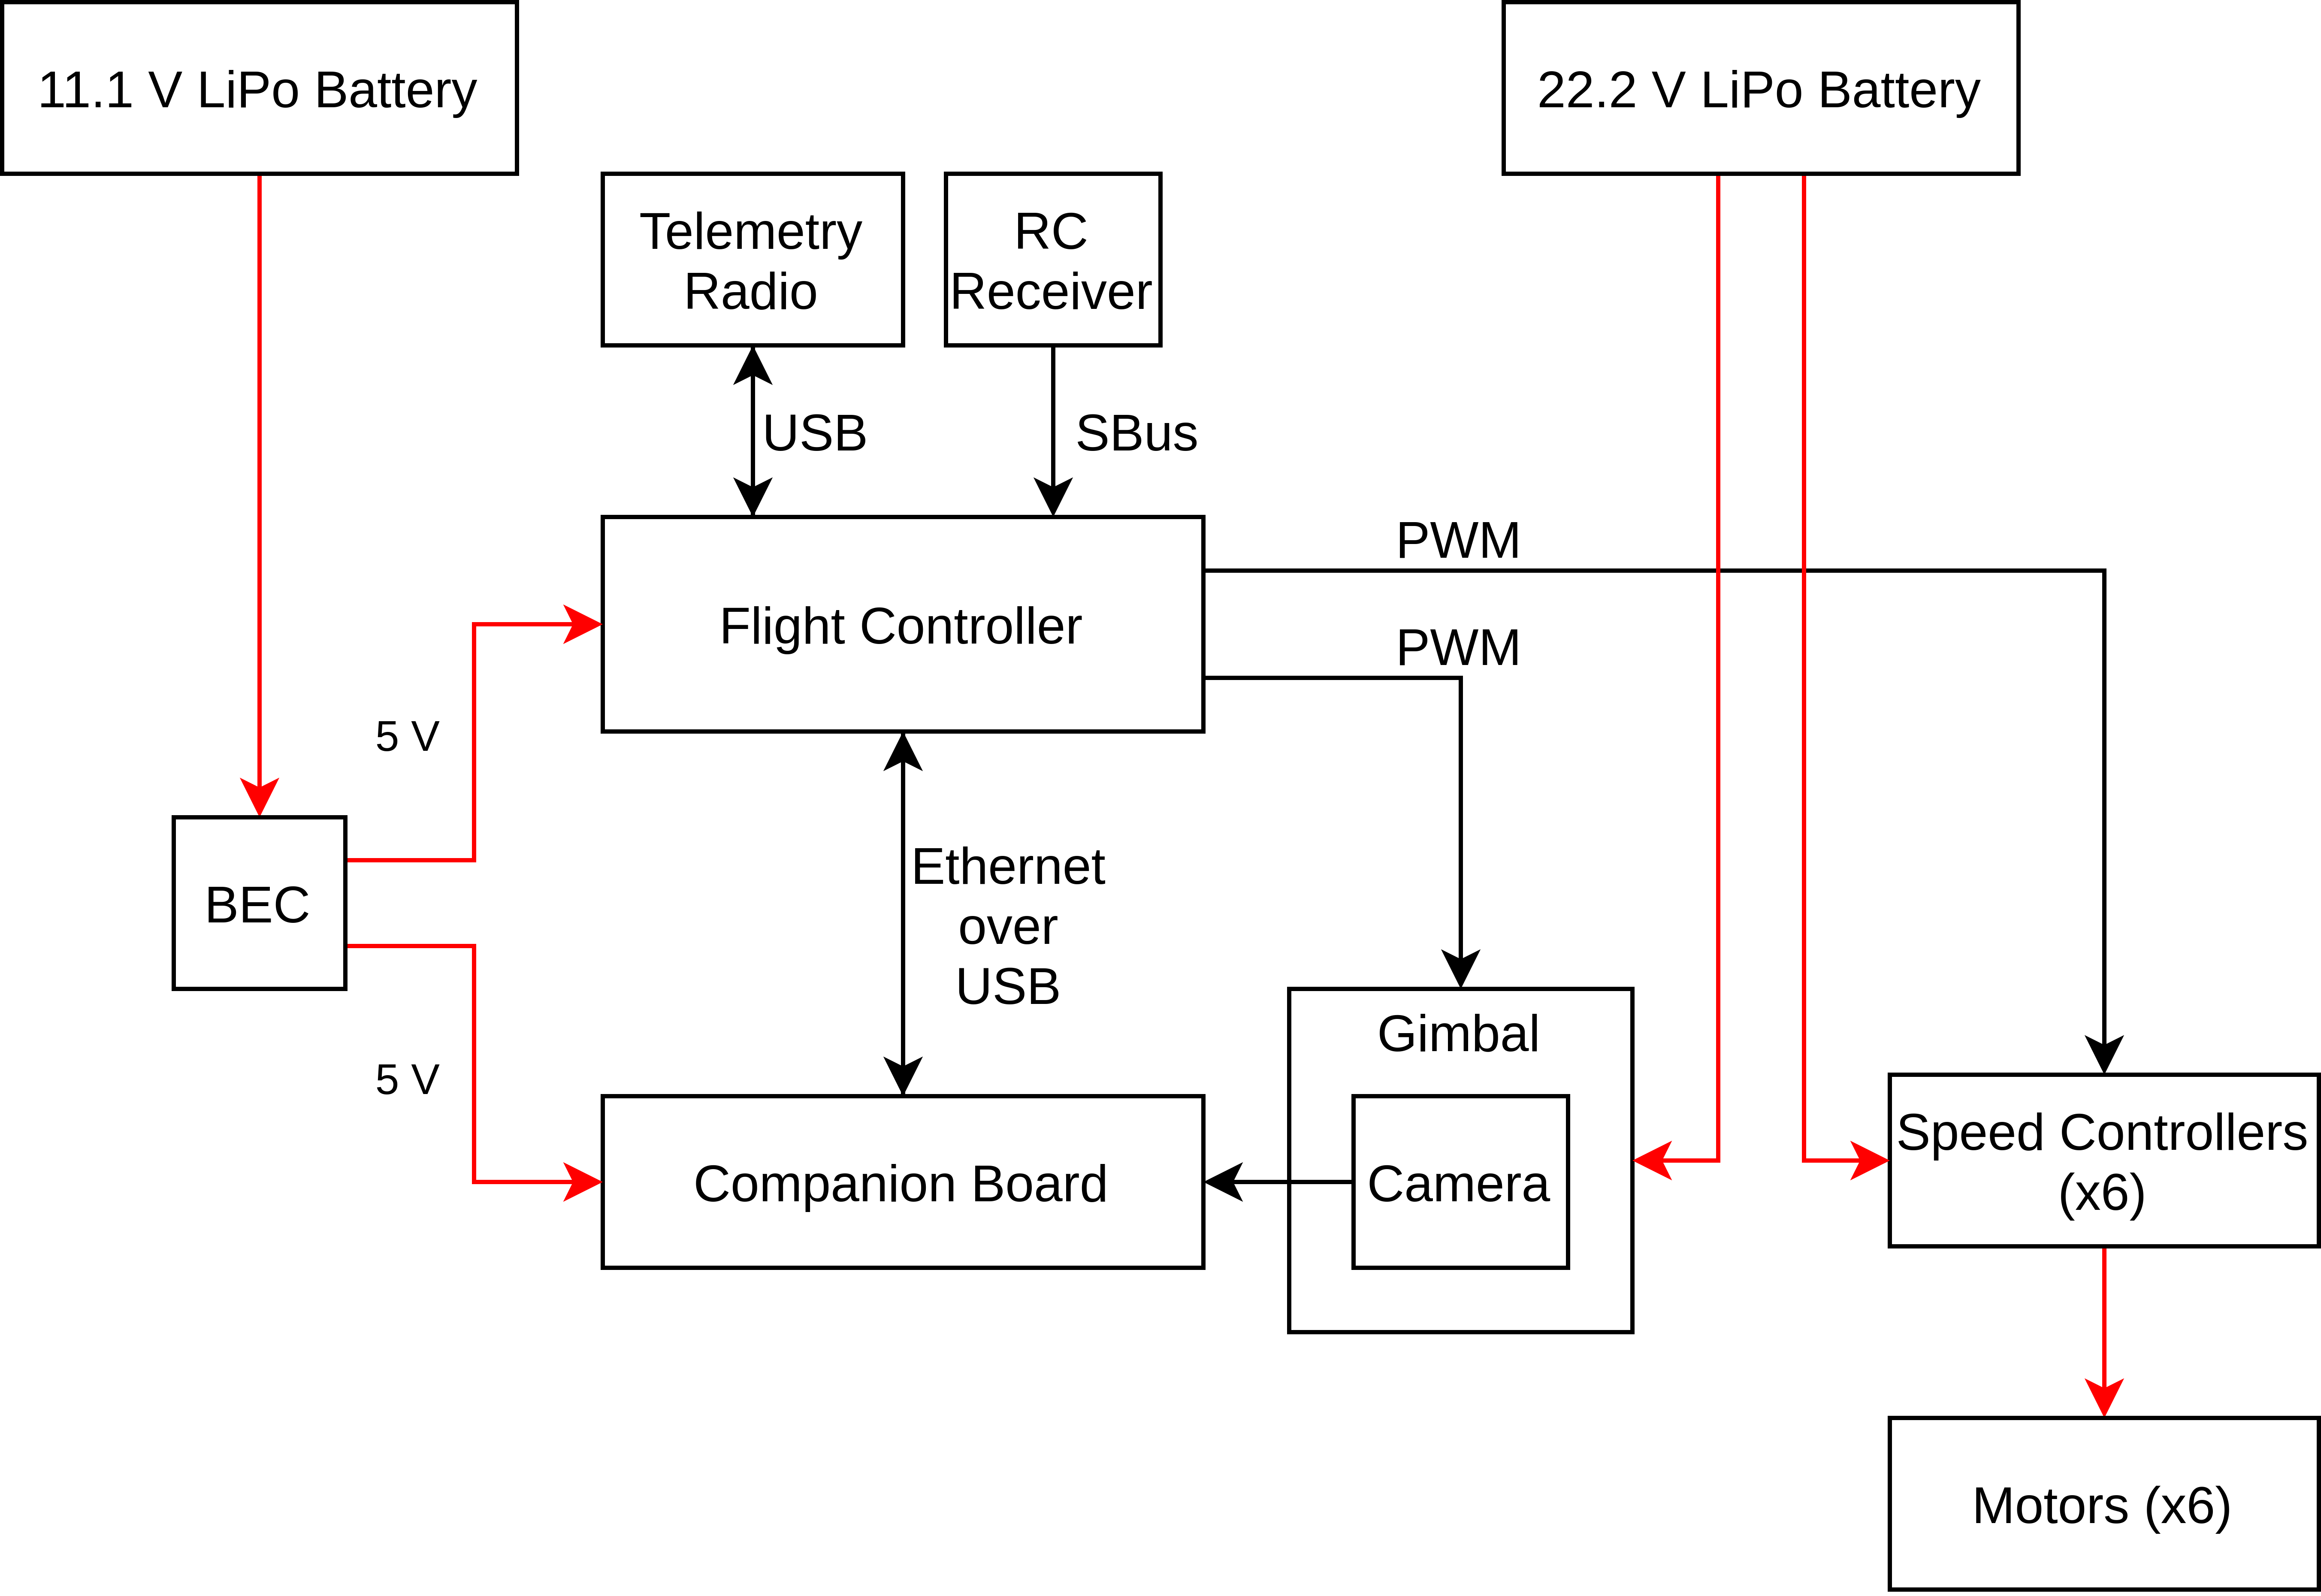
\includegraphics[width=0.7\linewidth]{hardware.png}
        \end{tikzfigure}

        Data flow for the autonomous landing task begins at the camera module, from which high-resolution video is fed into the companion board.
        A program \texttt{gscam} resizes the video to a lower resolution to reduce computational requirements, and pipes the resized video to the \texttt{whycon\_ros} module for analysis.
        The \texttt{landing\_controller} module performs coordinate system transforms to generate a target position for the drone based on the detected position of the landing pad.
        The \texttt{gimbal\_controller} module sends control signals (through the flight controller via the \texttt{rc/override} ROS topic) to the gimbal in order to center the landing pad in the camera's field of view.
        When no landing pad is detected, the gimbal is controlled manually by the operator.
        The \texttt{MAVROS} module receives information from the landing and gimbal controllers, translates it into lower-level commands, and passes those commands to the ArduPilot software.
        ArduPilot sends control signals to the gimbal and speed controllers to make the drone approach and track the landing pad.
        \begin{tikzfigure}
            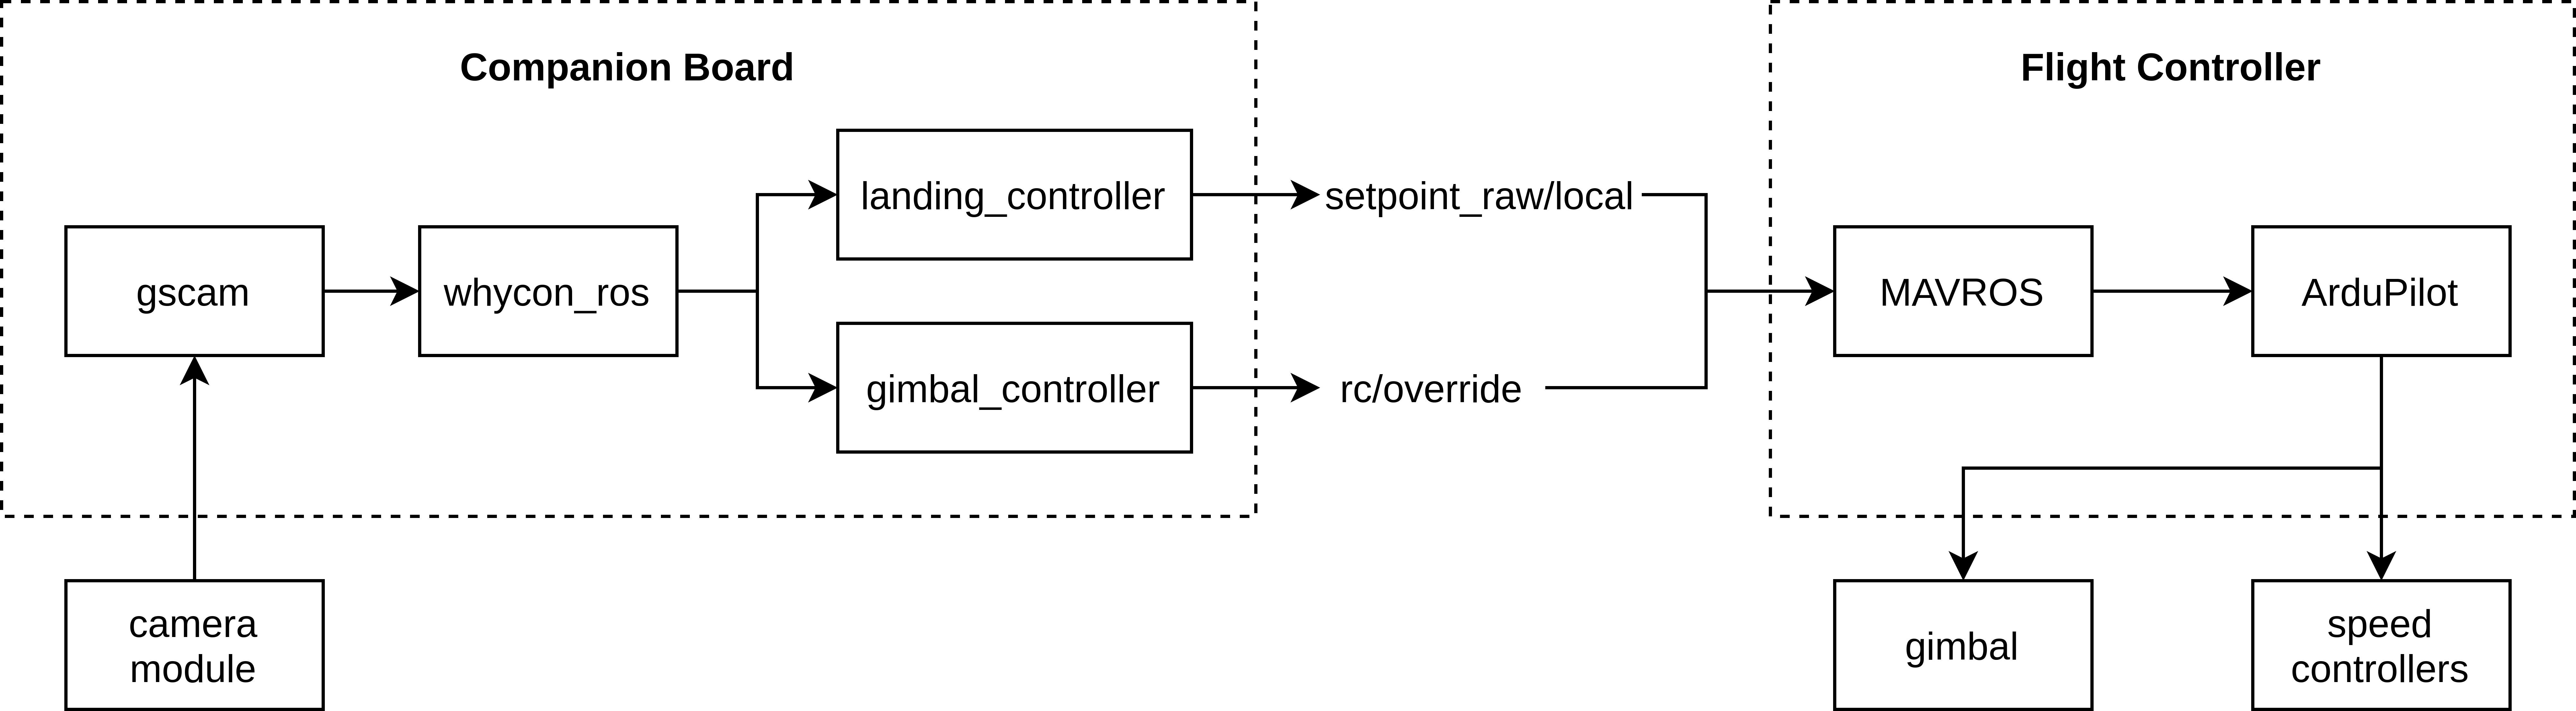
\includegraphics[width=0.7\linewidth]{data_flow.png}
        \end{tikzfigure}
    }

    \block{Landing Pad Design and Detection Performance}
    {
        \normalsize
        \begin{minipage}[t]{0.75\linewidth}

            Fiducial markers (top: April Tag\cite{apriltag_paper}, bottom: WhyCon\cite{whycon_paper}) allow the drone to determine its position relative to the landing pad using only a normal RGB camera.
            The larger WhyCon marker is easier for the system to recognize at long range, while the April Tag marker provides more accurate pose estimates at close range.
            The April Tag marker is positioned in front of the WhyCon marker in order to keep it in the field of view of the camera at close range.
            The drone touches down in the center of the WhyCon marker.
            After initial testing, the April Tag system required substantial computational resources on the companion board and was therefore removed.
            The final landing pad design includes only a WhyCon marker.
            Fig. \ref{fig:gimbal_controller_performance} shows the performance of the gimbal controller in aiming the camera at the landing pad in a 640x480 frame.
            These graphs show that the camera is successfully aimed at the landing pad (with some typical PID oscillation) in most cases.
            Cases where the landing pad is not fully centered are those where the gimbal reaches its rotational limits.
            The oscillation is a result of high PID gains (for quick correction) but does not adversely affect the detection performance.

        \end{minipage}
        \hfill
        \begin{adjustbox}{valign=t}
            \begin{minipage}[t]{0.2\linewidth}
%                \vspace{-1cm}
                \begin{tikzfigure}[Initial Landing Pad Design]
                    \fbox{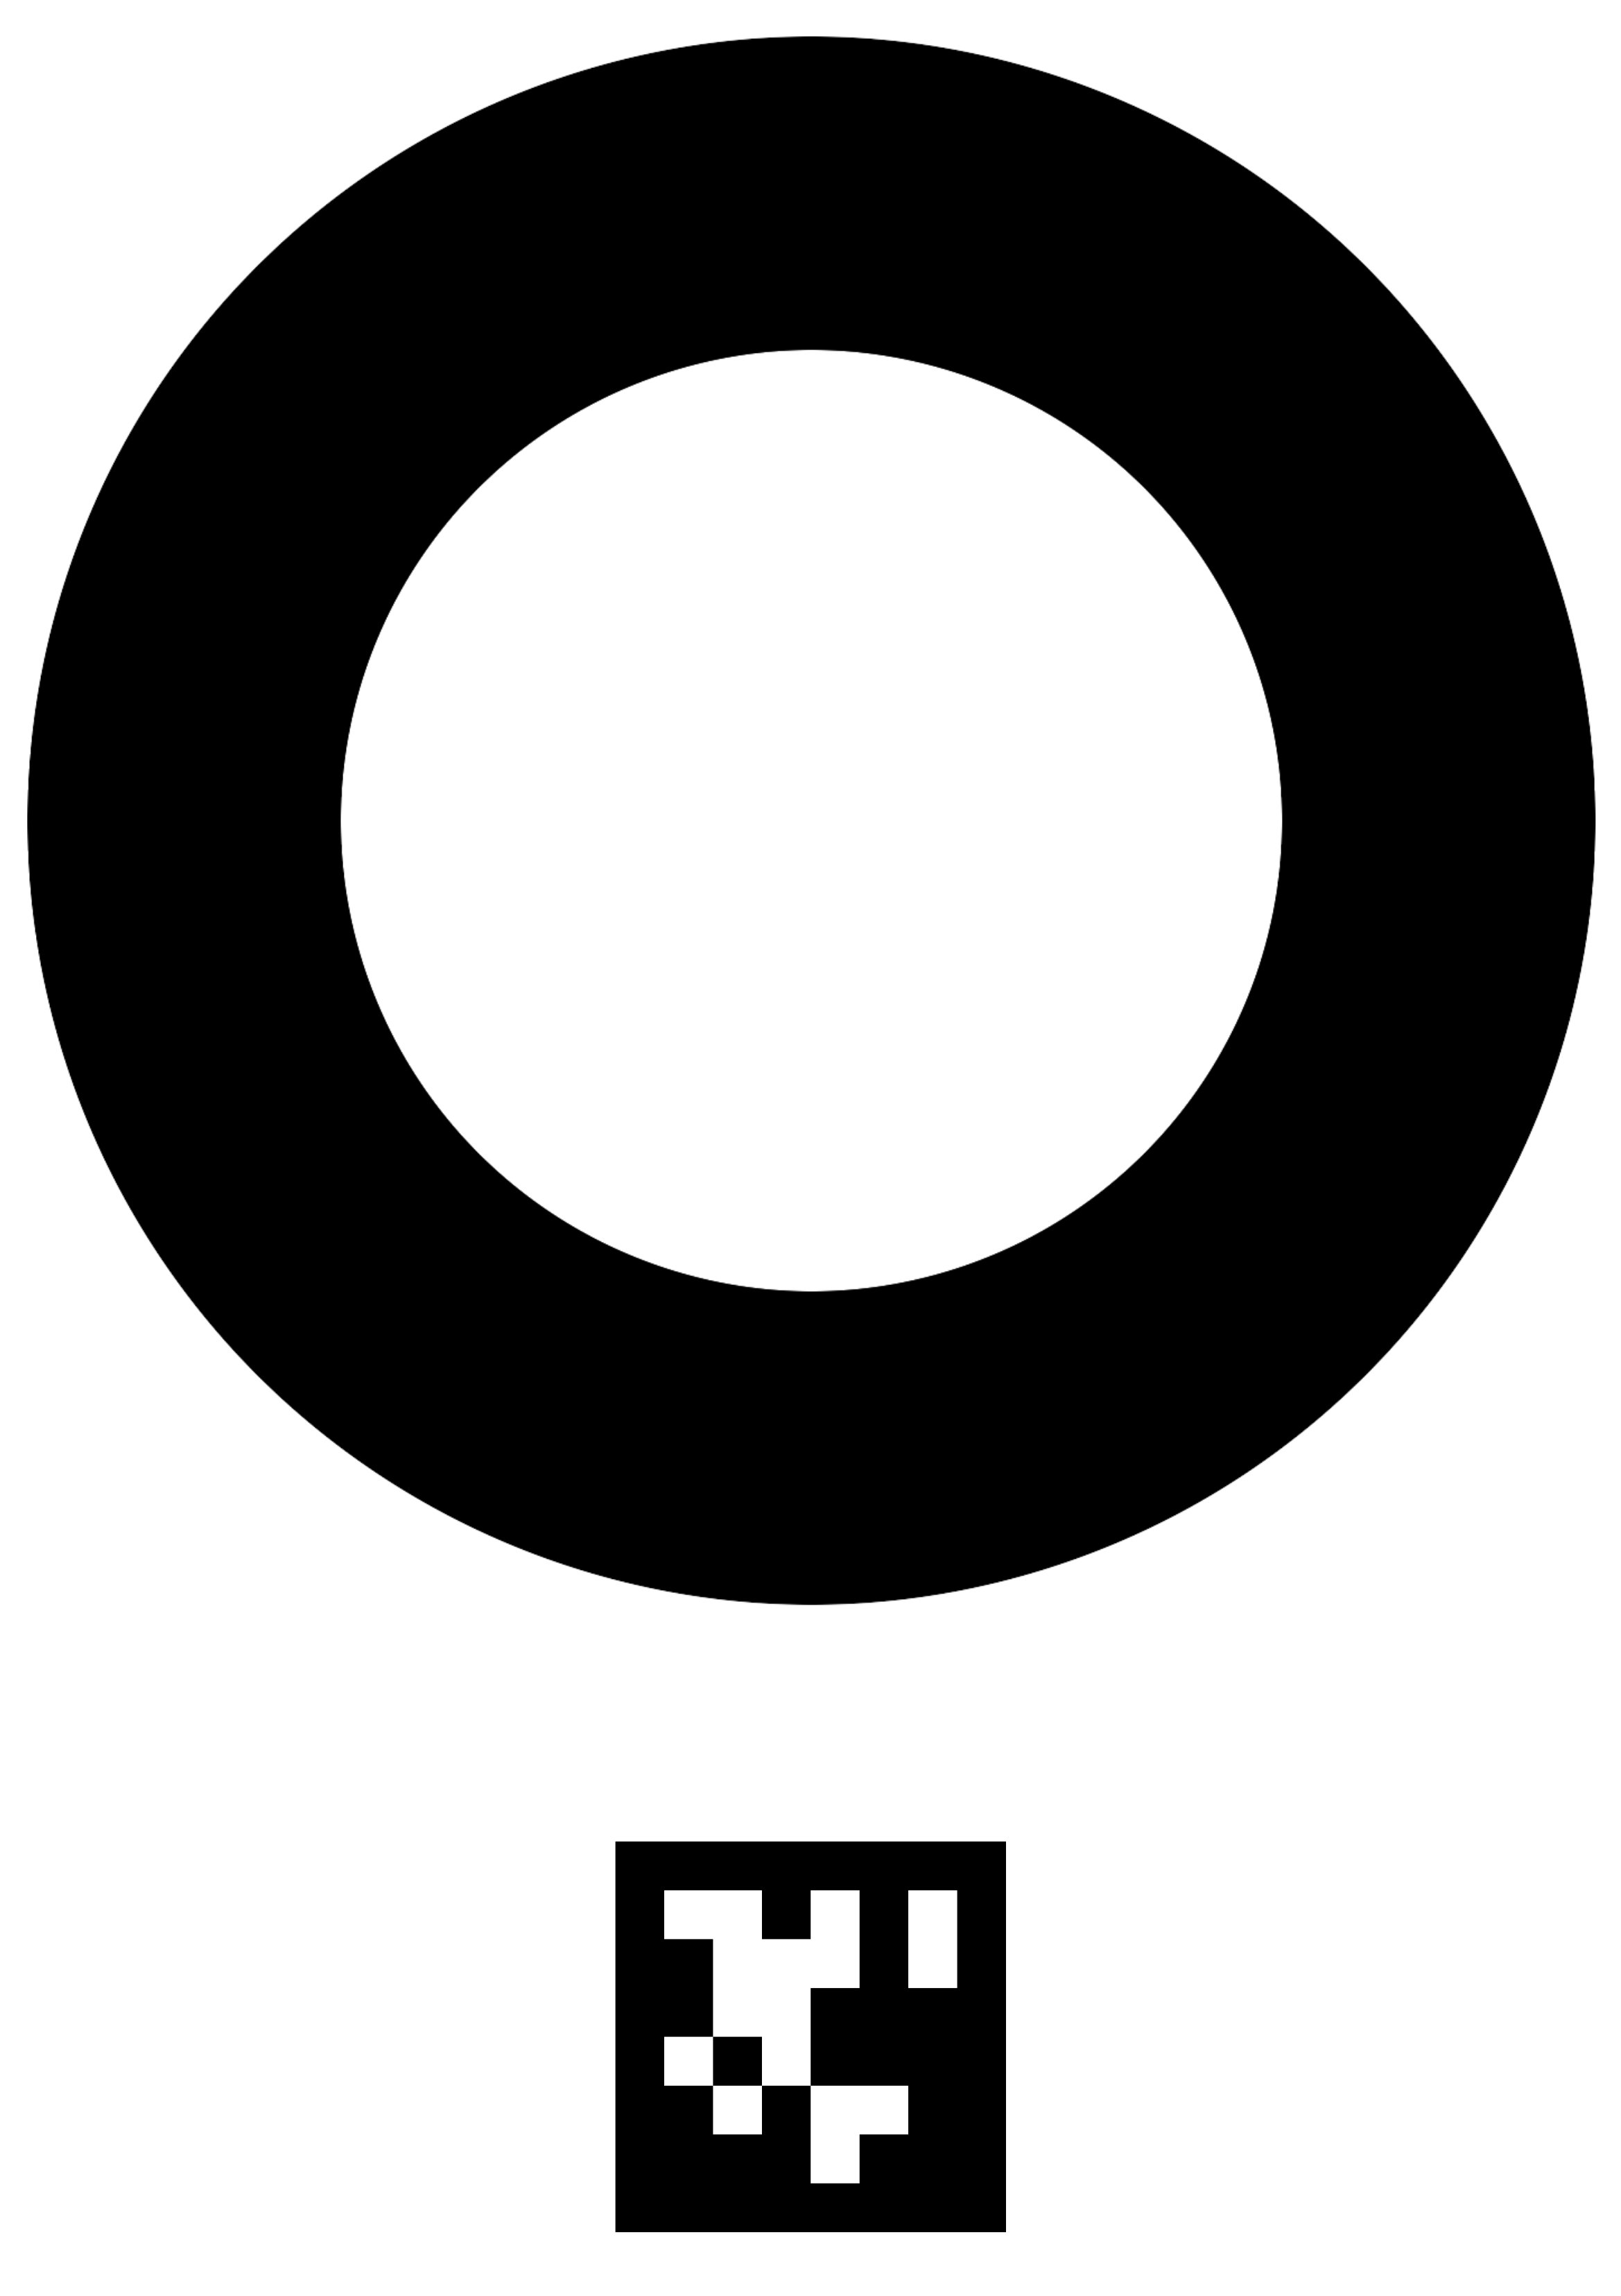
\includegraphics[angle=180, width=0.8\linewidth]{landing_pad.png}}
                \end{tikzfigure}
            \end{minipage}
        \end{adjustbox}

        \vspace{-0.5cm}
        \begin{tikzfigure}[Performance of Gimbal Controller in Centering the Landing Pad in the Camera's FOV]
            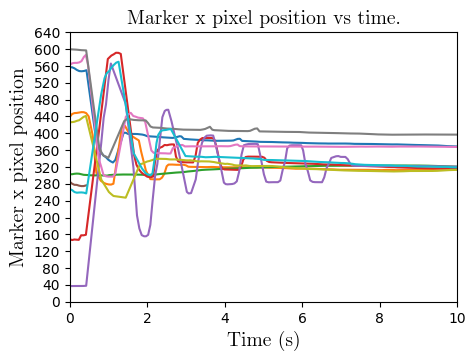
\includegraphics[width=0.45\linewidth]{coral_gimbal_performance_x_axis.png}
            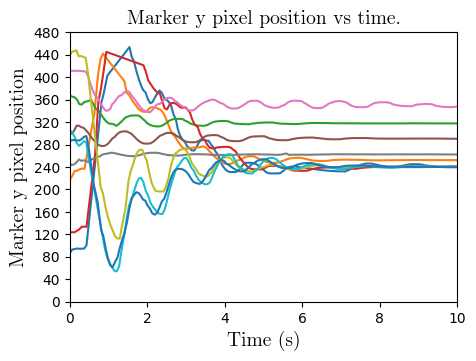
\includegraphics[width=0.45\linewidth]{coral_gimbal_performance_y_axis.png}
            \label{fig:gimbal_controller_performance}
        \end{tikzfigure}
    }

    \column{0.33}
    \block{Flight and Landing Performance}
    {
        \normalsize
        Both drones have stable and reliable performance even in high wind, with safe flight times of roughly 15 minutes.
        They have enough power to lift additional sensors/electronics.
        The cameras are able to aim at the landing pad reliably in a laboratory setting, however the Jetson Nano had power issues in field testing.
        The Google Coral drone was able to reliably aim the camera, generate position targets and approach the landing pad autonomously.
        Because of an issue with the WhyCon marker system, the pose estimation was inaccurate at close range and therefore landing was aborted at the last minute.
        However, this issue is not major and will be addressed in future work.
        Fig. \ref{fig:stability} visualizes the pitch, roll, and altitude performance of the drone during a hover of about 10 seconds.
        The pitch and roll vary by about 2.5 degrees (as normal) because of hardware performance and environmental conditions.
        The altitude varies by about 2 meters as a result of manual control. Fig. \ref{fig:drone_in_flight} shows the drone in flight.

        \begin{tikzfigure}[Pitch, roll, and altitude during hover.]
            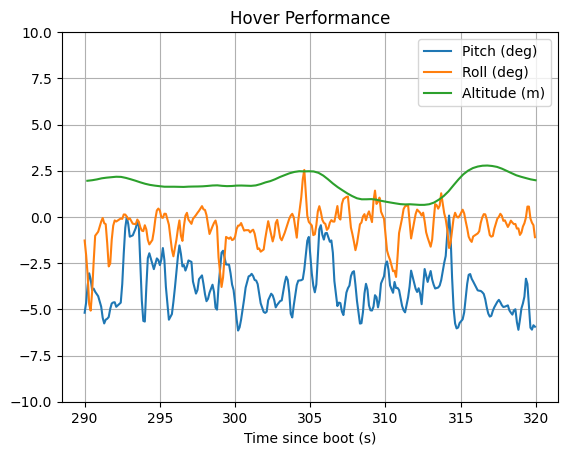
\includegraphics[width=0.45\linewidth]{stability.png}
            \label{fig:stability}
        \end{tikzfigure}

        \begin{tikzfigure}[Drone in Flight (Scan QR code in top right for video!)]
            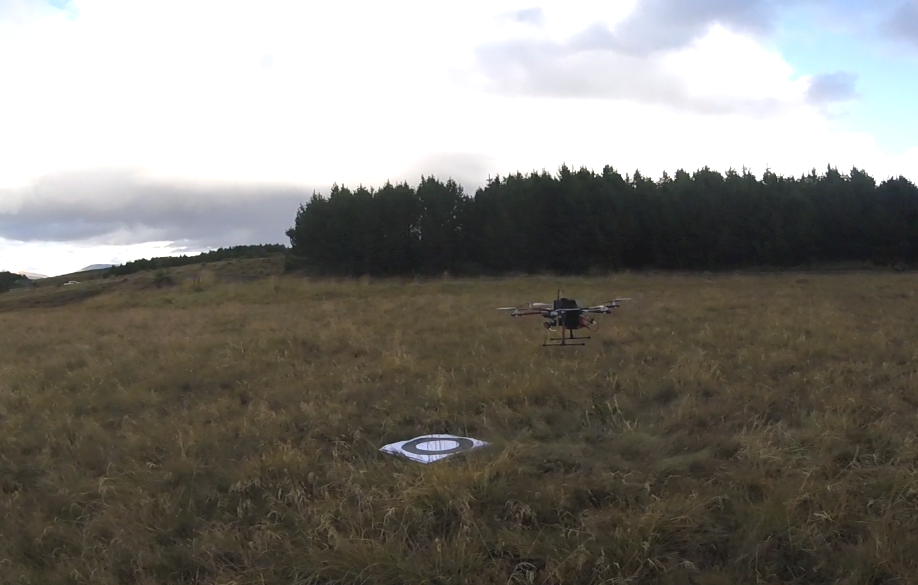
\includegraphics[width=0.6\linewidth]{drone_in_flight.png}
            \label{fig:drone_in_flight}
        \end{tikzfigure}
    }
    
    \block{Future Work}
    {
        \normalsize
        The pose estimation system will be changed to fix its issues that occur when the drone is at close range to the landing pad.
        One possible solution is to attempt to fix the WhyCon system itself.
        Another solution is to use existing deep learning models (ex.- EfficientPose or PoseCNN) to create a new pose estimation system, as the companion boards are designed for embedded deep learning tasks.\\

        The drones will be tested in different autonomous scenarios, such as more complex point-to-point missions.
        They will serve as flexible platforms for more specific tasks such as terrain mapping, object tracking, etc.
    }

    \block{References}
    {
        \printbibliography[heading=none]
    }

\end{columns}
\end{document}